\documentclass[a4paper]{jpconf}
\usepackage{graphicx}
\usepackage{array}

\usepackage{etoolbox}



\newcolumntype{C}[1]{>{\centering\let\newline\\\arraybackslash\hspace{0pt}}m{#1}}
% \usepackage{citesort}
\bibliographystyle{iopart-num}
\newcommand{\BibTeX}{Bib\TeX}
\newcommand{\REVTeX}{REV\TeX}

\begin{document}

\title{Multy-cascade enrichment schemes for reprocessed uranium recycling}
\author{V E Gusev}
\address{National Research Nuclear University “MEPhI”, Department of Molecular Physics, 115409, Russia, Moscow, Kashirskoe shosse, 31}
\ead{gusevvlad13@mail.ru}

\begin{abstract}
This paper deals with the problem of reprocessed uranium (RepU) enrichment in cascades of gas centrifuges with simultaneous fulfillment of requirements on concentrations of isotopes $^{232,234,236}$U. These harmful isotopes bred by nuclear chain reaction are responsible for an increase in radioactivity level and neutron poisoning of fresh nuclear fuel.
The study examines the cascade schemes that aim at closing the nuclear fuel cycle by satisfying the formal condition of the complete uranium reclaim. The prospective VVER fuel cycle strategy of multiple uranium recycling is considered. Schemes under consideration are multi-cascade ones. Such configurations are necessary to fulfill both a series of requirements on concentrations of even-numbered isotopes in commercial low-enriched uranium and condition of 'full return' of uranium extracted from spent nuclear fuel from particular reactor to produce fresh fuel load for the same reactor.
The research provides a basis for comparison between three various multi-cascade schemes designed to re-enrich RepU under mentioned above conditions. I used the unified metrics (related to ordinary cascade and normalized to LEU product) of natural uranium savings, separative work, and depleted uranium consumption and their derivative. The calculations take into account the necessity of RepU dilution to compensate for the adverse effects of $^{232,234,236}$U isotopes. As the reference cascade scheme, a simple modification of a single triple-flow cascade for RepU enrichment was considered. It is demonstrated that some modern cascade schemes could provide sustainable recycling of uranium.
\end{abstract}

\section{Introduction}
As the Russian nuclear industry is expanding with its VVER-type pressurized water reactors, the issues with the nuclear fuel cycle (NFC) should be resolved in advance. First, spent nuclear fuel (SNF) should be dealt with as its accumulation accelerates. Second, the resources of fissile uranium that is used for VVER fresh fuel production should be secured. That must be done while taking into account the nuclear non-proliferation measures, international standards, and economic efficiency. Rosatom plans to achieve that by implementing the closed NFC with fast neutron reactors. Though on the way to this far-reaching goal the NFC should be closed partially through fuel recycling in VVERs.\\
If we want to recycle SNF, it should be reprocessed to withdraw the valuable components that can be reused. It leads us to uranium and plutonium, which make up approximately 93\% and 1\% of irradiated fuel, respectively. In this study I consider the application of uranium recovered separately -- reprocessed uranium (RepU).\\
In order to produce fresh nuclear fuel for VVER -- low-enriched uranium (LEU) -- we need to increase the percentage of $^{235}$U in uranium mixture to about 4\% in the composition. As natural uranium contains 0.71\% of $^{235}$U, we need to achieve more than a five-fold increase of this fissile isotope. The modern separation technology -- cascades of gas centrifuges -- successfully performs this enrichment operation.\\
Reprocessed uranium contains about 1\% of fissile $^{235}$U (more than a stock one mentioned above), but it has some undesirable features -- the artificial $^{232,236}$U and an extra $^{234}$U. These even-numbered isotopes spoil the isotopic composition with additional radioactivity and neutron poisoning \cite{Hida2017, Coleman2010}.\\
As a consequence, we need to deal with special requirements that limit their concentrations and provide a surplus of $^{235}$U in LEU \cite{extra1}. Moreover, the RepU re-enrichment strategy will demand the exact ratio of its consumption per unit of product. To manage the turnover of fissile materials, the SNF to LEU proportion should be set at 1:1. Furthermore, this should be repeated round and round to maintain multiple recycling. All in all, the presence of even-numbered isotopes presents a challenge for RepU recycling. The basic scheme, where the raw material is just fed to the three-flow conventional cascade, is not capable of meeting the necessary conditions anymore. To overcome this, some modifications were proposed \cite{Prusakov2008,Palkin2013,Sulaberidze2006,doi:10.1063/1.5099598,Palkin2015,Palkin2017,Palkin2016}. Some of them uptake the depleted uranium (DepU), helping in the reduction of its huge stockpiles \cite{Smirnov2014}.

\section{Materials and Methods}
In this paper, we compare a set of cascades designed to return the regenerated uranium to NFC. We consider a case when the scheme produces the equivalent amount of LEU product to recycled used fuel. To simulate multiple recycling of nuclear fuel, we apply as a RepU feed an isotopic composition that has already undergone five consecutive cycles. The key characteristics related to overall efficiency, such as natural uranium (NatU) savings, separative work expenses, and energy spending, were evaluated for each scheme. All these values were normalized to the resulting LEU (per unit of product). Then, they have been taken in relation to their equivalents in the basic cascade (three-flow cascade for NatU enrichment).
In order to avoid cost indicators, we used the methodology for recalculating material flows (NatU savings, the volume of enriched wastes and separative work units) into units of energy consumed (megawatt hours)  \cite{rodionovaAnalizTehnikoekonomicheskihHarakteristik2019a}. This metric has been proposed as a universal assessment tool for cascades that re-enrich uranium. 

\subsection{Schemes of cascades}
Let us give a quick review of the analyzed schemes.
In cascade No.1 (Fig. \ref{1}) the feeds are mixed before the entry. The satisfactory LEU product could be made only for the relatively pure isotopic composition, given the condition of full reclaim. The scheme leads to SW losses owing to mixing the compositions (at the very beginning) with different concentrations. The same is true for all the `mix' signs on the drawings.\\
The next configuration No.2 is a multi-cascade scheme (Fig. \ref{2}). The fist basic three-flow cascade here enriches the feed slightly higher than it is required for the LEU product, which then will be purified from $^{232,234}$U a bit by depletion. Then, the second cascade accumulates the LEU in its `heavy' end, while the lightest $^{232,234}$U (along with a great deal of $^{235}$U) are dragged to the other side as a waste).
The double scheme No.2 is altered to the form of No.3 (Fig. \ref{3}) \cite{MEPhI2018}. This design provides a complete return. This condition is fulfilled by adding the proper LEU from the cascade 3. The absence of $^{232}$U in this supplement allows producing reactor-grade fuel that satisfies all the requirements on even-numbered isotopes. The main drawback here is that it generates the unacceptable byproduct marked as `Toxic waste' in Fig. \ref{3}.
The cascade No.3 is then modified to No.4 (Fig. \ref{4}) \cite{doi:10.1063/1.5099598} to blend down the toxic waste by DepU. This straightforward strategy solves the serious problem of radioactive waste treatment. At the same time, it retains the valuable $^{235}$U that could have been discarded (its fraction in light end of the second cascade comes close to that of HEU (20\% or higher concentration of $^{235}$U)). It should be noted that the second cascade of schemes No.2-4 faces the radioactive contamination due to the build-up of $^{232,234}$U.

\begin{figure}[h]
\begin{minipage}{10pc}
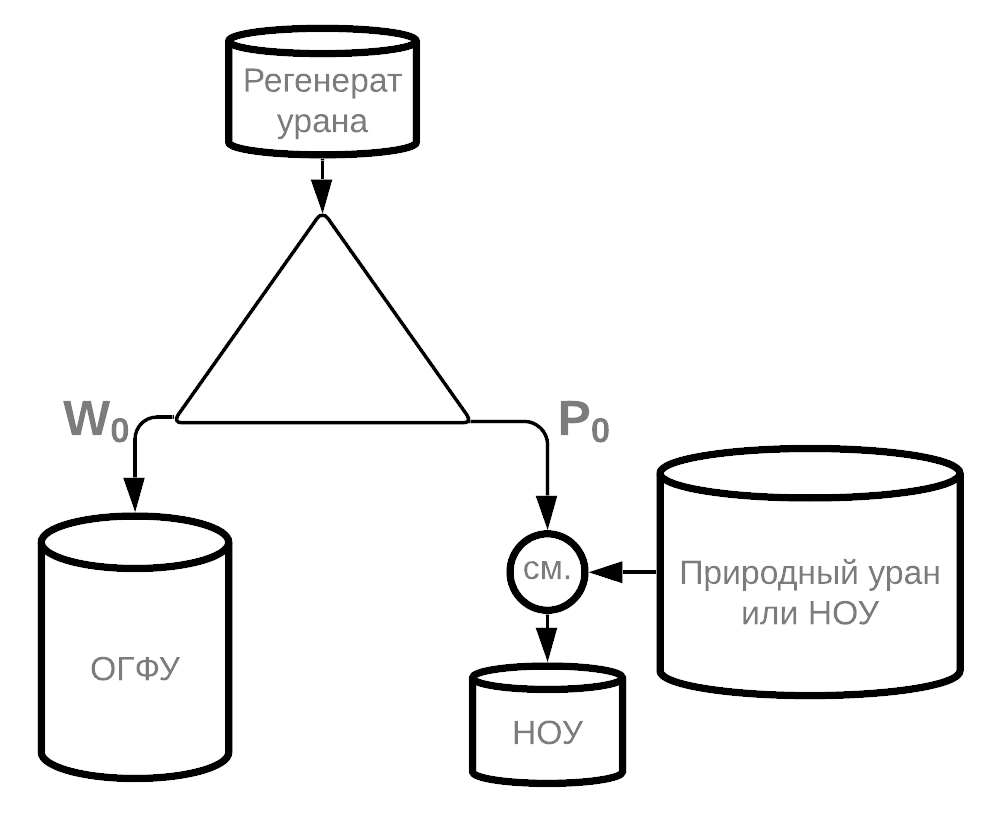
\includegraphics[width=10pc]{1.png}
\caption{\label{1}Scheme No.1.}
\end{minipage}\hspace{1pc}%
\begin{minipage}{11pc}
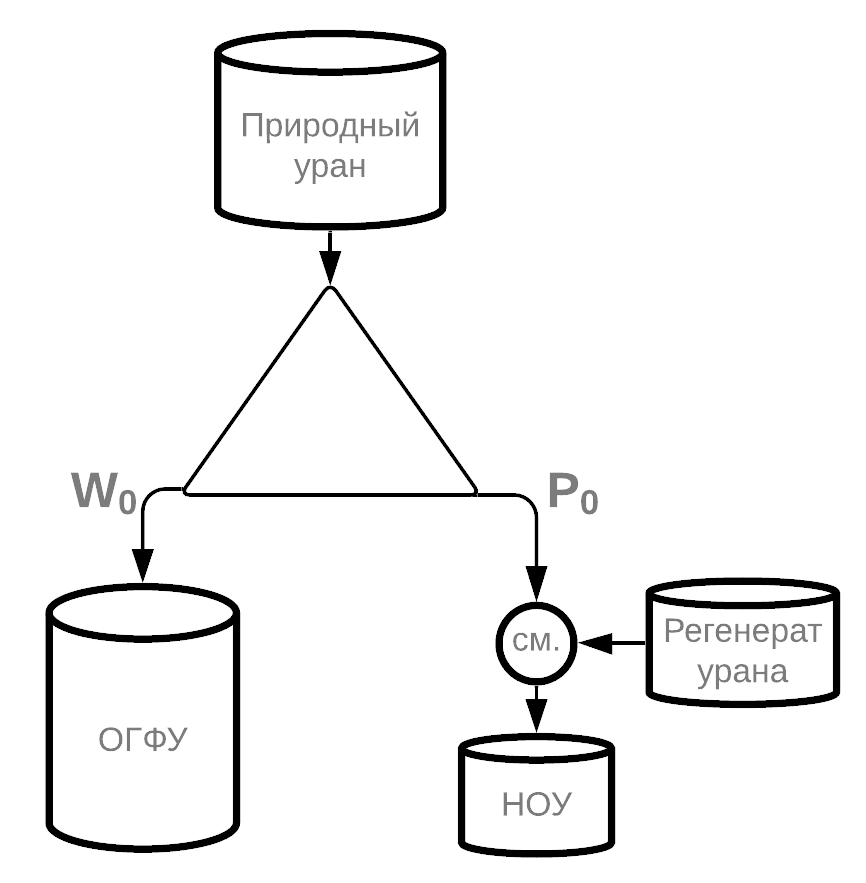
\includegraphics[width=11pc]{2.png}
\caption{\label{2}Scheme No.2.}
\end{minipage}\hspace{1pc}%
\begin{minipage}{15pc}
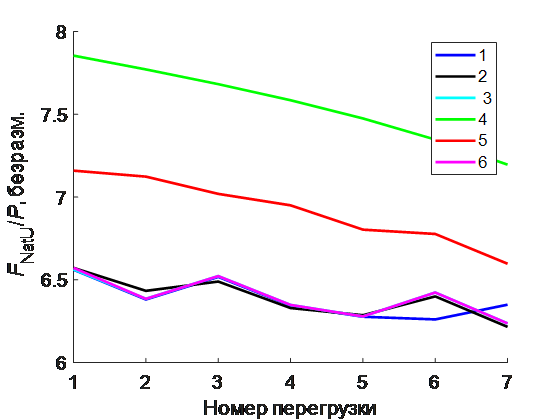
\includegraphics[width=15pc]{3.png}
\caption{\label{3}Scheme No.3.}
\end{minipage}
\end{figure}

\begin{figure}[h]
\centering
\begin{minipage}{16pc}
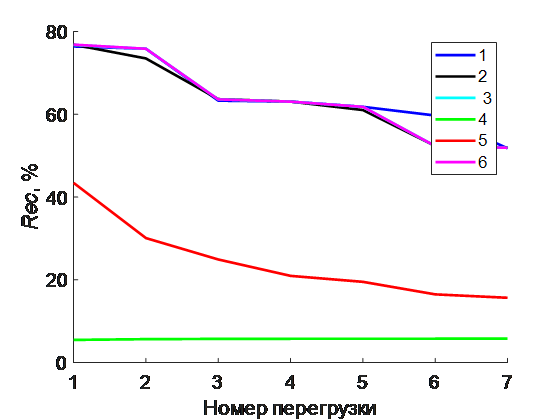
\includegraphics[width=16pc]{4.png}
\caption{\label{4}Scheme No.4.}
\end{minipage} 
\end{figure}

\subsection{Mathematical model and main assumptions}
\begin{table}[h]
\caption{\label{composition}The isotopic composition of spent fuel from VVER-1000.}
\begin{center}
\begin{tabular}{1111111}
\br
Mass number&232&233&234&235&236&238\\
\mr
Concentration, \% &1.0258\cdot10$^{-6}$&1.3017\cdot10$^{-6}$&3.9067\cdot10$^{-4}$&1.0675&1.4458&97.4476\\
\br
\end{tabular}
\end{center}
\end{table}

In this paper, we used the cascade model with a non-mixing condition for the chosen pair of components (Matched Abundance Ratio Cascade), which is a subset of quazi-ideal cascade \cite{DelaGarza1977, Sulaberidze2001}. The separated mixture is enriched by centrifugation in the form of gaseous uranium hexafluoride, which is the typical working substance for uranium isotopic composition \cite{refId0, orlov2015}. The RepU feed is an isotopic composition that has been recycled five times (Table \ref{composition}). This choice allows us to simulate the condition of multiple reuses of uranium fuel). Separation factor for $^{232}$UF$_{6}_$ to $^{238}$UF$_{6}_$ is 1.2 \cite{MEPhI2018}.\\
    In LEU product: required concentration of $^{235}$U -- 4.7\%, $^{232}$U is limited by $5\cdot10^{-7}$\% (as supposed to be permitted in VVER in the future), $^{234}$U to $^{235}$U ratio must not exceed 0.02, $^{236}$U poisoning effect is balanced out (compensated) with $^{236}$U$\cdot0.29$ of additional fissile $^{235}$U. Reprocessed uranium consumption per unit of the LEU product equals 0.93 (fraction of uranium recovered from SNF) to satisfy the 1:1 condition \cite{MEPhI2018}.\\
The $^{235}$U concentration in the product flow of the second cascade is limited by 19.99\% (to stay in the low-enrichment uranium category). For each cascade with index 2, the `backing' component is $^{236}$U, and $^{238}$U for the others. It should be reminded that the `target' component is always $^{235}$U.\\
The SWU overconsumption ratio for scheme No.4 (Fig. \ref{4}) is fixed at the levels of its increase by a quarter and by half (comparing to ordinary scheme for natural uranium enrichment). In this scheme, the DepU supplement to the feed of the fourth cascade refers to the low-grade tails made of natural uranium with a concentration of $^{235}$U = 0.1\%. Note, that using the material of higher $^{235}$U concentration (ordinary tails with about 0.2\% of $^{235}$U) would lead to less SWUs needed.\\
The depleted uranium output has the same $^{235}$U concentration equals to 0.1\%, but the additional cascade with index 4 of scheme No.4 (Fig. \ref{4}) has a single stage in its depletion side, so that the newly yielded DepU has slightly less concentration of $^{235}$U. 

\section{Results and discussion}
\begin{table}[h]
\caption{\label{results}Summary table for comparison of cascades.}
\begin{center}
\begin{tabular}{1|C{1.5cm}C{2.5cm}C{2.5cm}C{2.5cm}C{2.5cm}}
\br
Cascade&NatU savings,\%&SWU overconsumption,\%&RepU rel. consumption&Rel. consumption of DepU&Theoretic rel. cost, \%\\
\mr
1&7.31&1.04&0.49&0&92.71\\
2&100&41.63&8.26&0&0.32\\
3&10.07&6.08&0.93&0&89.96\\
4&15.08&25&0.93&31.11&85.00\\
4&23.13&50&0.93&74.49&77.02\\
\br
\end{tabular}
\end{center}
\end{table}

The No.1 (Fig. \ref{1}) scheme is not capable of yielding the needed RepU/LEU ratio for repeated recycling. This happens because of the `dirty' initial composition of RepU (that was already recycled several times). However, we should pay tribute to its ability to retain some natural uranium at the expense of minor separative work losses. As a result, we get more than 7\% gain in cost.\\
Despite the 100\% saved natural uranium and, hence, the low relative cost, scheme No.2 (Fig. \ref{2}) failed to meet the requirements on $^{232}$U thus leaves the competition.\\
Results show that the gain in NatU economy (and, as a consequence, in rel. cost) goes with the extra expenses on SW. Schemes No.3,4 (Fig. \ref{3},\ref{4}) could provide the desired ratio of RepU intake hence formally close the NFC (in reality, it is just a partially closed fuel cycle). No.4 (Fig. \ref{4}) gives the highest results in NatU preservation that could be enhanced further with additional SWUs. It happens due to the DepU wide-scale involvement. The No.4 is the only scheme from the sample that reverses the accumulation of burden (composition high in $^{232}$U and $^{235}$U).
The collateral `mobilization' of depleted uranium requires additional expenses of SWU, but overall beneficial as long as the stockpiles of this material are a headache itself \cite{3fc8fca6fe0546ca9319d4bf1a6127a3}. Overall, this increase in separative work goes with a rel. cost decrease, as natural uranium economy has a higher impact in the examined framework.\\
All the schemes, except No.2, produced LEU of the formally equivalent commercial quality.

\section{Conclusion}
The paper discussed the issues of complete uranium return to the NFC and doing it in a sustainable way, that, in other words, means achieving repeated recycling. The means of simultaneously meeting all the requirements have been considered along with the challenges of toxic wastes accumulation and strict limitations on even-numbered isotopes. The latest cascade scheme is capable of resolving all these problems at the expense of additional SWU consumption. Moreover, this way is cheaper in terms of energy units, which comprised the most important practical characteristics of enrichment cascade.


\AtEndEnvironment{thebibliography}{
\bibitem{extra1}Kislov A I Titov A A Dmitriev A M and Sintsov A E, {\it Nuc. Rad. Saf.} 52–59 (in Russian)}
% настроить нумерацию

\section*{References}
\bibliography{iopart-num}



%Допустимо не сокращать название и приводить список авторов до 10 человек

\section*{Acknowledgments}
The study was carried out with the support of the grant from the Russian Science Foundation (project No.18-79-00249).
\end{document}


